\section{Overview}

Historically, the study of atmospheric-pressure plasmas (\acs{app}'s) is
indistinguishable from the study of plasmas as a whole. However, the detail of
the measurements and calculations associated with \acs{app}'s has been limited
by their complexity. From a computational perspective, the high pressure and
number of potential reactions present a difficult challenge. Likewise, the high
pressure can significantly complicate the data analysis for a number of plasma
diagnostics. Aside from the high pressures, the large electric fields, short
time scales, and general randomness of \acs{app}'s make even the most basic
observations a feat.

In the last several decades, some of this has begun to change. High-powered
computing has allowed simulations with remarkable detail. Similarly, advances in
technology has enabled plasma diagnostics in regimes that were experimentally
inaccessible. As a result, the body of knowledge regarding \acs{app}'s has
greatly increased. Sometimes, the motivation for this work is scientific
curiosity. More often, the study of \acs{app}'s has been driven by a broad range
of applications.

Among the first plasma applications were provided by \acs{app}'s: ozone
generation and lighting. Aside from these items, plasma welding, polymer
treatment, combustion, and plasma televisions have become widely accepted.
Meanwhile, a large number of new applications may soon be added to this list,
including: treatment of tissue wounds, altering airflow over airfoils, and
destruction of industrial pollutants.

Unsurprisingly, each case demands a different kind of plasma. The original arc
discharges were created between two graphite rods connected to immense battery
banks. In contrast, a modern research reactor studying plasma-assisted
combustion might use a fast-switching semiconductor circuit. Over the years,
several types of \acs{app}s have been developed for a variety of situations:
dielectric-barrier, corona, thermal arc, RF, microwave, pulsed, and more.

Within this group\footnote{The interested reader is referred to Starikovskaia's
review \cite{Starikovskaia2006} which provides a general overview of \acs{app}'s
in the context of plasma-assisted combustion}, the repetitively-pulsed
nanosecond discharge (\acs{rpnd}) has created considerable interest. Generally
speaking, a \acs{rpnd} is a plasma generated by a repetitive electrical pulse
applied between two electrodes. The pulse voltage is often in excess of one
kilovolt, lasts anywhere from $<1-100$ ns, and is repeated over a thousand
times each second. The result is a wave of ionization (and light) which crosses
from the powered electrode to the grounded one.

A \acs{rpnd} can fill volumes of several liters with a relatively uniform
plasma. Though they can cause significant excitation of the background gas, they
generally produce very little heating (in some cases below a detection limit of
$\Delta \pm 15$ K). In addition, the excitation can be changed with adjustments
to the magnitude or duration of the electrical pulse. Each of these
characteristics are highly desirable in one or more of potential applications
for \acs{app}'s.

Given all of these promising properties, \acs{rpnd}'s have been the subject of
substantial study by several research groups. However, much of this work has
focused on the physics of \acs{rpnd}'s in air. Unfortunately, air's large number
of constituent elements can lead to notable complexity. In turn, this can
obscure some of the more fundamental questions relation to \acs{rpnd}'s: how do
they form, how is the energy distributed between excited particles, and what
kind of spatial variation can be expected?

This paper details a study of each of these questions in a helium \acs{rpnd}.
Specifically, the densities of one particular excited atom are measured for a
variety of pressures and locations. This is complemented by measurements of the
light emissions for the same set of parameters. A simple model of a \acs{rpnd}
is used to predict several characteristics of the plasma based on the excited
state densities: electron density, electric field, and light emission. The
measured light emissions are interpreted to show how the energy is distributed
in the gas, and how it changes over time. Finally, they are compared with the
estimated light emissions to check the validity of several common assumptions.

The remainder of this chapter is comprised of a review of the associated
literature, as well as a discussion of basic discharge theory. Chapter
\ref{chp:exp} covers the experimental setup as well as some general observations
of the \acs{rpnd}. Next, the measurement of the excited state densities is
presented, followed by the chapter on the light emission measurements. Chapter
\ref{chp:model} explores the global model used to interpret the excited state
densities, as well as some supporting particle-in-cell simulations. Finally, the
paper concludes with a discussion of how the models and measurements impact the
present understanding of \acs{rpnd}'s.

\section{Literature Review}

\acs{rpnd}'s are only a recent invention which resulted from advances in
fast-switching semiconductors. However, they belong to a category of plasmas
which have formation times much shorter than can be explained by the familiar
Townsend mechanism. Included in this category is lightning, some sparks,
streamers, and others. These plasmas cover several disciplines, and as a result,
the method of formation has acquired several different names. Here, we adopt the
phrase, fast ionization wave (\acs{fiw})\footnote{It should be noted that the
phrase wave does not indicate any kind of periodic motion or spatial
arrangement. Simply put, it describes a boundary which separates ionized and
unionized gas which travels from one electrode to another.}.

Perhaps the first recorded observation of an artificial \acs{fiw} was the work
of Thomson \cite{Thomson1893}. In his work, Thomson made a measurement of a
``luminous front'' which moves through a long and narrow glass tube, as seen in
Figure \ref{fig:thomson}\footnote{Though Thomson's work was inspired by
measurements that Wheatstone had made in 1835 \cite{Wheatstone1835}, it is not
clear that Wheatstone's apparatus was actually generating a \acs{fiw}.}.
\begin{figure}
  \centering
  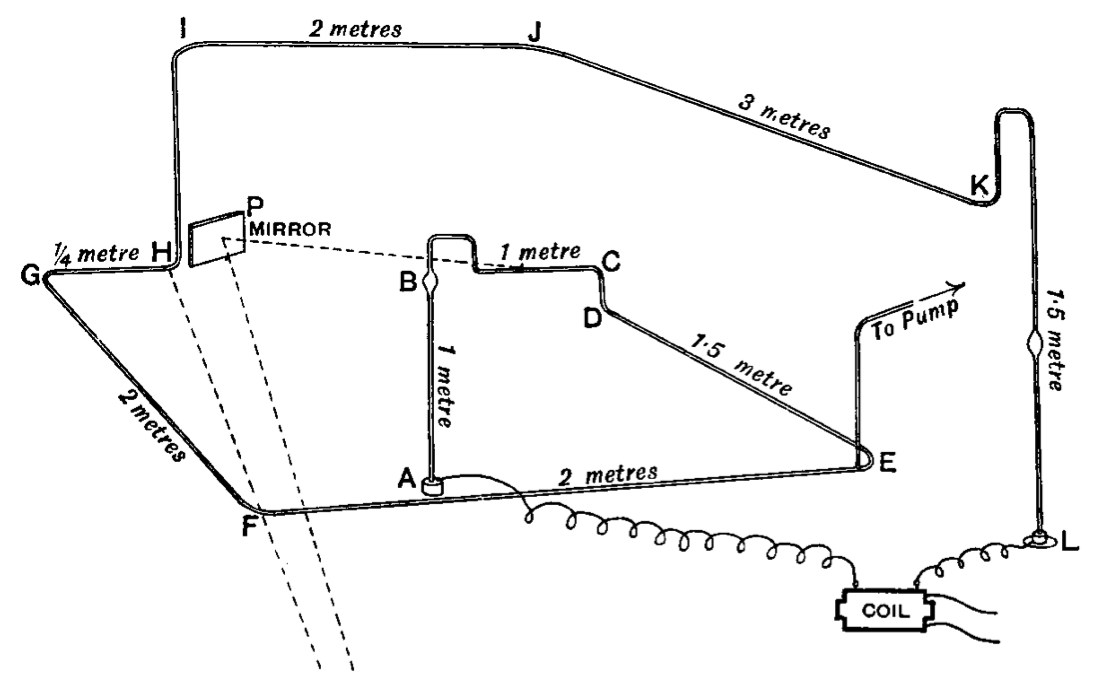
\includegraphics[width=4in]{chapters/introduction/figures/thomson.png}
  \caption{A sketch of J.J. Thomson's early experiments on fast ionization
  waves in long vacuum tubes.}\label{fig:thomson}
\end{figure}
Thomson noted that the velocity of the luminous front had a speed approaching
$1\times10^{10}$ cm/s. Furthermore, he observed that the front travelled from
the positively pulsed electrode (anode) to the ground electrode (cathode).

Thomson examined the sensitivity of the \acs{fiw} to various electrode shapes
and materials, but found that it was qualitatively unchanged. In 1930, Beams
made a critical change to Thomson's original experiment. In contrast to
Thomson's work, Beams applied a \emph{negative} pulsed to one electrode, and
held the other at ground. He observed that the \acs{fiw} travelled from the
cathode to ground, opposite the direction that Thomson had observed
\cite{Beams1930}.

The discovery of quantized charge and verification of the electron's existence
in 1897 \cite{Thomson1897} provided Beams the opportunity to make the first
detailed interpretation of an \acs{fiw}. His qualitative description of the
\acs{fiw} formation remains accurate, even now:
\begin{quote}
  In the neighborhood of the electrode $\ldots{}$ the field is very high and
  intense ionization should take place. This ionization due to the large
  difference in mobilities of positive ions, negative ions and electrons
  respectively should result in the establishment of a space charge. This space
  charge, once formed near the high potential electrode $Q$ must move down the
  tube regardless of the polarity of the applied potential because of the
  changes it produces in the field near its edges.
\end{quote}
In other words, the motion of the \acs{fiw} is a result of a moving electric
field gradient associated with the build up of space charge.



Simultaneous studies of lightning emphasized its similarity to sparks, first
noted by Benjamin Franklin. 

Around the same time, there was a distinct set of researchers ho were studying
similar phenomena in lightning. In most cases, these studies concentrated on
time-resolved photography, pioneered by Boys\footnote{In the same article, Boys
anticipated a number of other atmospheric physics studies by proposing that
rockets be fired at thunderclouds. Unfortunately, he lived in a village of
thatched houses and could not conduct the experiment for fear of
fire.}\cite{Boys1926}, and refined by Schonland \cite{Schonland1935}. This
technique was later adopted by Allibone and Meek \cite{Allibone1938} to observe
the evolution of a laboratory-generated spark.

By 1935, fast ionization waves had been under study for nearly 50 years.
However, there was still no adequate explanation for the speed of the discharge.
Similarly, Beams' observation that the wave always travelled from the high
voltage to the low voltage electrode (regardless of polarity) was inconsistent
with the Townsend model used to explain most plasmas. Based on observations made
with fast pulses, Flegler and Raether developed a new theory of breakdown for
sparks in air \cite{Flegler1936} which was capable of, at least partly,
explaining the fast ionization wave phenomena. Independently, Loeb and Meek
developed a similar theory in 1940 \cite{Loeb1940}.

The work of Fleger and Raether as well as Loeb and Meek, was intended to explain
the breakdown processes for an undetermined range of overvoltages (in excess of
the breakdown voltage). However, as early as 1951, Fisher and Bederson
\cite{Fisher1951}, demonstrated that the Townsend mechanism was still plausible
at low overvoltages.

In contrast, 1961 saw Fowler \cite{Fowler1961} seeking a hydrodynamic
explanation for the waves. Contrary to the stochastic and particle-based
description of the streamer breakdown, Fowler considered the luminous fronts to
be nonlinear electron acoustic waves. Though the explanation provided a fair
agreement with his observations, Loeb \cite{Loeb1965} identified several
issues with the analysis, namely an overly simplified geometry and resultant
reduction in the estimate field strengths.

By 1965, Loeb himself, admits that photoionization was not insufficient on its
own to produce the observed phenomena. In his review for Nature, Loeb
identified several phenomena that exhibited similar characteristics. The
return stroke in lighting, high overvoltage breakdown in rarefied gases, and
sparks in atmosphere. Loeb was able to provide a qualitative description of the
physics involved, but ultimately deferred on any quanitative description.

The insufficiency of photionization was later reinforced by the observation of
Mesyats \cite{Mesyats1972} that the speed of the discharge processes was often
faster than the lifetimes of excited states. Again, this precluded
photoionization from providing a significant amount of preionization for the
propagation of an rpnd. Mesyats instead suggested that the large fields
generated an electron avalanche that grew much more rapidly than the typical
Townsend discharge. This was followed by an avalanche chain which further
propagated the plasma.

This explanation 

Later, Kunhardt \cite{Kunhardt1980} extended on Mesyats' analysis and provided a
more theoretical underpinning for it. Taking his inspiration from the group
theory used in neutron diffusion, Kunhardt explored the development of a fiw
from the perspective of ``trapped'' and ``runaway'' electrons. In his
work, Kunhardt identifies th

Previous work by
Babich and Stankevich \cite{Babich1973} inspired this by suggesting the
existence of continually-accelerated electrons at high overvoltages.

As an aside, the topic of electron beams in rare gases became of substantial
interest to researchers in the mid 1970s. Because rare gases lacked low-lying
excited states which might detrimentally absorb energy, they were favor for
laser where a population inversion could be achieved with ease. As a result, a
great deal of work went into detailing the propagation of an electron beam in
rare gases which is physically similar to the development of a fast ionization
wave. However the primary difference between

It was around this time that the topic of fiw became of substantial interest to
Russian research groups. Though much of the early work is shrouded in the mists
of language differences, it is believed that Vasilyak \cite{Vasilyak1994}
provides a fair review of the material. 

Come 1998, the fiw was the subject of renewed interest by a group of researchers
at the Moscow Institute of Physics and Technology \cite{Anikin1998}. They
employed several different diagnostic techniques (photomultiplier tubes and
capacitive probes) in an exceptionally detailed study of fiws in both air and
nitrogen, using a shock tube and a bell jar. A summary of these investigations
can be found in \cite{Starikovskaia2001}. The work showed exceptionally
reproducibility of the discharge parameters at relatively low repetition rates,
on the order of tens of Hz, and evidence of runaway electrons in the
electronically excited molecular states. This work also included some of the
first approximations of the electron energy distribution function (\acs{eedf}).
This was found by comparing several paremeterized distribution functions with
the resulting excited state populations. 

This was time the population kinetics of an fiw was really examined. In this
case, it emphasized the short-lived states of nitrogen. Specifically,
\cite{Pancheshnyi1998} initially used the fiw to examine the population of
electronic states of nitrogen. Later analysis \cite{Pancheshnyi1999} concluded
that the, for a negative fiw in nitrogen, the vast majority of the electrons
were generated in the aftermath of the wave and that the ionization did not
track the luminous front. Additionally, measurements of the conductivity
suggested that the local approximation becomes invalid in the wave front and the
electron energy distribution function resembles a beam.

The development of fid semiconductor technology in the late 1990's and their
commercialization in the early 2000's allowed the use of rpnds. Fundamentally,
these discharges were the same as the fiws that had been studied for decades
earlier. However, the much greater repetition rates (on the order of tens of
kHz), meant that the discharges could be used in a number of previously
impossible applications. Attention quickly turned toward plasma-assisted
combustion \cite{Starikovskaia2006}, mhd energy bypass \cite{Macheret2002}, and
later, plasma actuators \cite{Adamovich2009}. Additionaly studies, related to
the development of high-pressure xenon lamps, led to several more quantitative
models of the fiw development \cite{Nikandrov2008, Tsendin2009}. These works
also contributed to a semi-analytical energy coupling model as well
\cite{Adamovich2009}.

Research efforts continued to use many of the same diagnostics as before. The
current and voltage at the powered electrode were recorded (with varying levels
of diligence), electric fields were measured with capacitive probes, and
photomoultiplier tubes were used to measure the progress of the luminous front.
The 2000's did add a few new tools to the diagnostic arsenal. Perhaps the most
common addition is the use of ICCD's in order to record transition and broadband
light. This approach has been used to verify the reproducibility of the
discharge \cite{Adamovich2009}. Though the gate times are still too short to
capture the development of the wave, excitation profiles like those initially
demonstrated by Vasilyak\cite{Vasilyak1994} are commonly recorded. Another, more
exotic addition, has been the use of CARS. This nonlinear technique has proven
to be excellent at reproducing the spatial temperature profiles of pulsed
nanosecond discharges. This has become particularly interesting for groups
interested in applications to fast gas heating \cite{Zuzeek2010}. Others have
used CARS to explore the electric field development of rpnds \cite{Ito2010,
Ito2010a}. Finally, another research group has used LCIF to detect the radial
and axial profiles of the metastable and electron densities in a helium
discharge. The CARS and LCIF approaches are both notable for being active
diagnostics of direct properties. This allows unprecedented time resolution and
detail.



